\documentclass{article}
\usepackage[utf8]{inputenc}
\usepackage{graphicx}

\title{Reporte 2: Fibonacci\\Iterativo vs Dinamico vs Recursivo\\\textbf{Análisis de Algoritmos}}
\author{ Ramiro Estrada García\\2015190034 }
\date{19 de Noviembre del 2020}

\begin{document}
\maketitle
\vspace{5cm}
\section {Características del PC}
\begin{itemize}
	\item CPU: Intel Core i5 9700F a 4.1GHz
	\item RAM: 16GB a 2666MHz
\end{itemize}
\newpage
\maketitle
\subsection{Iterativo}
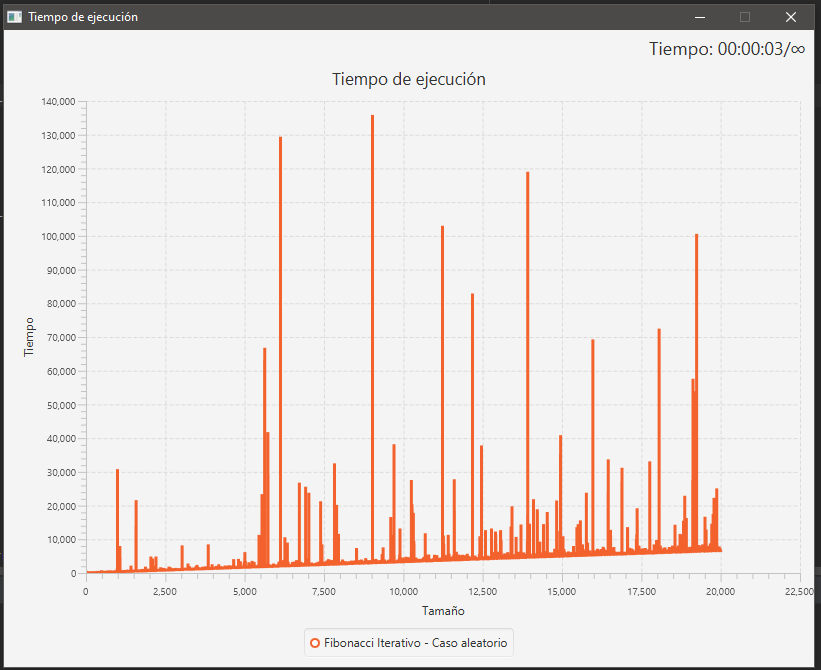
\includegraphics[width=12cm]{iterativo.png}\\
\subsection{Recursivo}
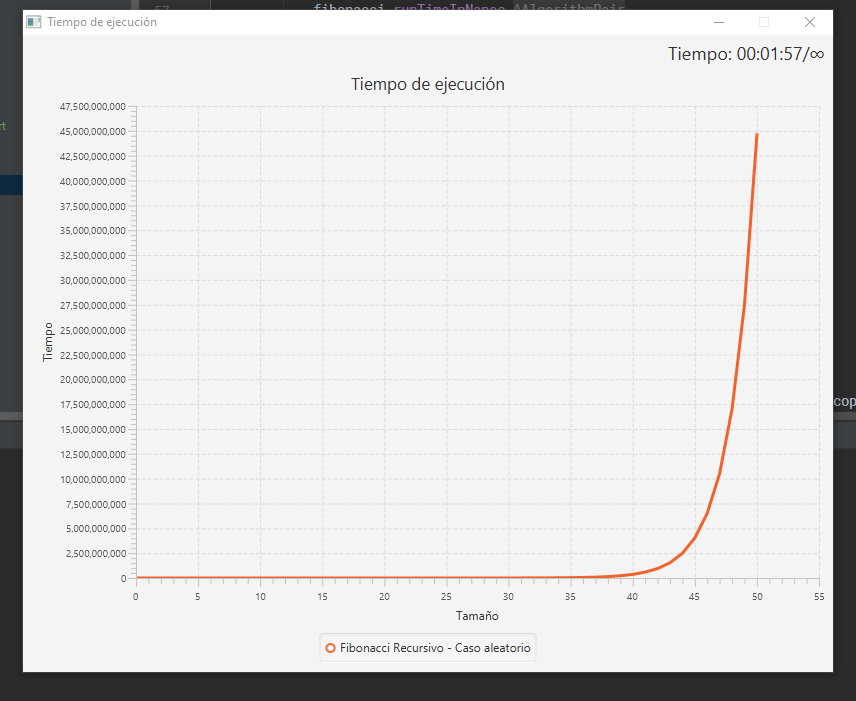
\includegraphics[width=12cm]{recursivo.png}\\
\subsection{Dinamico}
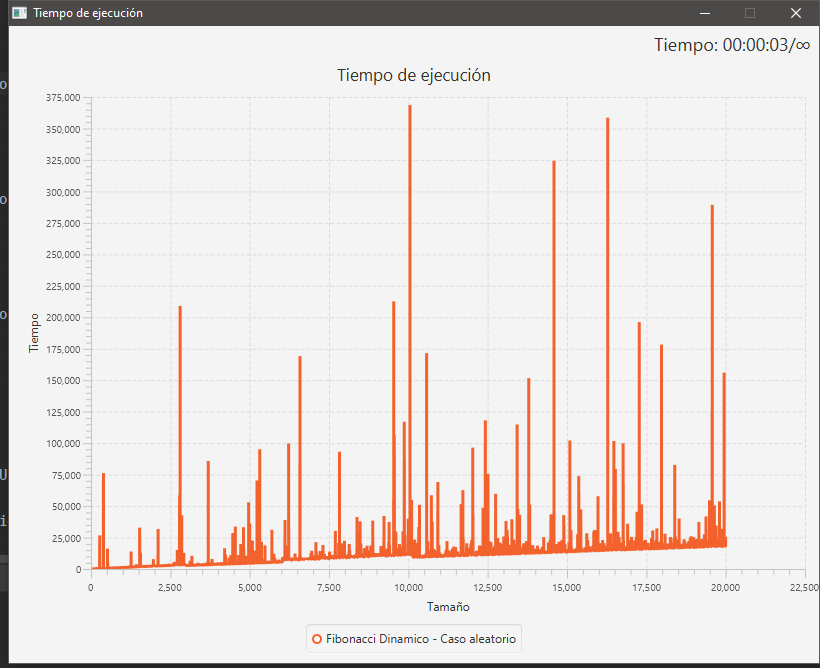
\includegraphics[width=12cm]{dinamico.png}\\
\section{Resultados}
En las graficas se puede observar diferentes comportamientos de los
acercamientos a resolver el problema de Fibonacci, en el caso del Dinamico
y el Iterativo los cresimientos son lineales teniendo mejor rendimiento el 
Iterativo con menor crecimiento. En el caso del recursivo se ve un cresimiento
exponencial gracias a que tiene que rehacer operaciones siempre que sean
necesarios.
\end{document}